\documentclass{article}
\usepackage{pgfplots}
\usepackage{siunitx}
\usepackage[paperheight=2.9in,paperwidth=3.9in,margin=0in]{geometry}
\pgfplotsset{compat=newest}
\usepgfplotslibrary{external}
\usetikzlibrary{patterns}
\tikzexternalize

 \definecolor{pastelred}{rgb}{1.0, 0.41, 0.38}
\definecolor{pastelmagenta}{rgb}{0.96, 0.6, 0.76}\definecolor{pastelpink}{rgb}{1.0, 0.82, 0.86}

\begin{document}
\pgfplotsset{
    every axis plot/.append style={line width=1pt, font=\large,}
}
 \pagenumbering{gobble} 
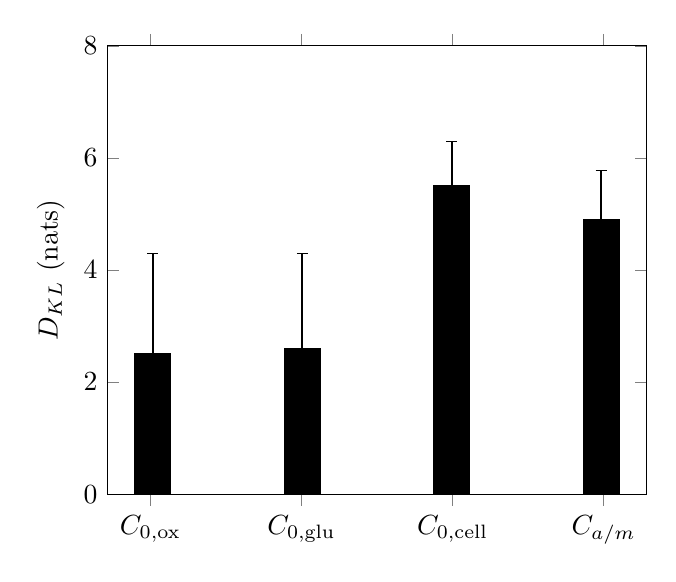
\begin{tikzpicture}
    \begin{axis}[
        ybar,
        ylabel = {$D_{KL}$ (nats)},
        ymin=0, ymax=8,
        xmin=0,xmax=5,
        bar width=13pt, 
        legend columns=2,
        xtick={0.4,1.8,3.2,4.6},
        xticklabels={$C_{0,\text{ox}}$,$C_{0,\text{glu}}$,$C_{0,\text{cell}}$,$C_{a/m}$},
         legend style={/tikz/column 3/.style={column sep=5pt},at={(0.53,0.97)}, anchor=north, font=\small }] 
                
        \addplot [ybar, fill=black, error bars/.cd,y dir=both,y explicit, error bar style={thick}] plot coordinates {
                (1, 2.5)+- (1,1.8)
                }; 
        \addplot [ybar, fill=black, error bars/.cd,y dir=both,y explicit, error bar style={thick}] plot coordinates {
                (2, 2.6)+- (2,1.7)
                }; 
        \addplot [ybar, fill=black, error bars/.cd,y dir=both,y explicit, error bar style={thick}] plot coordinates {
                (3, 5.5)+- (3,0.79)
                }; 
        \addplot [ybar, fill=black, error bars/.cd,y dir=both,y explicit, error bar style={thick}] plot coordinates {
                (4, 4.9)+- (4,0.88)
                };        

     \end{axis}
\end{tikzpicture}
\end{document}               

        




